
\chapter{Background}
\textit{This chapter serves two main purposes. Firstly, it evaluates the available literature surrounding the effectiveness of techniques for modelling, control and state estimation in unmanned aerial vehicles and related platforms. Secondly, it introduces to the key mathematical, physical and technical concepts necessary for the discussion in the following chapters.}

\section{Modelling Multi-Rotor Vehicles}
\subsection{Modelling Approaches}
In order to control a system, it is first necessary to have an understanding of the dynamics of the system. There are multiple methods used for developing mathematical models in order to describe the dynamics of multi-rotor vehicles. The Newtonian approach uses forces and torques in order to describe the system, whereas the Lagrangian approach utilises energies\cite{Raine2017}.\\

 Further, attitude of the vehicle can be described by using either Euler angles or quaternions. Euler angles express attitude with three angles, each representing the rotation in 3D space around each axis. Alternatively, quaternion algebra is used to represent attitude with 4 scalar variables representing a point on the unit sphere\cite{Voight2021}. Euler representation is more intuitive, however quaternion representation has the advantage of avoiding a problem known as gimbal lock which arises when two of the Euler rotation axes align, resulting in a loss of a degree of freedom.\\

Newton-Euler formalism combines Newtonian mechanics and Euler angle representation in order to describe the rotational and translational dynamics of rigid bodies. This approach is commonly used to develop a mathematical model for multi-rotor vehicles. The main advantage of this method is that it is simple to understand. 


Alternatively, using Euler-Lagrange formalism results in a more compact derivation\cite{Zhang2014}. \\

%Linearisation...

\subsection{Newton-Euler Equations}
The Basic Kinematic Equation (BKE) is used in Newton-Euler dynamics to describe the relative motion of two reference frames \cite{Ardema2006}. The BKE is given in Equation \ref{eqn:BKE1}:
\begin{equation}\label{eqn:BKE1} 
\frac{d\textbf{Q}_{a}}{dt}=\frac{d\textbf{Q}_{b}}{dt}+\omega_{b} \times \textbf{Q}_{b}
\end{equation}
where $\textbf{Q}_{a}$ and $\textbf{Q}_{b}$ represent a 3 dimensional quantity (e.g position, velocity) with respect to reference frames \{A\} and \{B\} respectively, and $\omega_{b}$ represents the angular velocity of \{B\} with respect to \{A\}. Now, consider reference frame \{B\} to be fixed at the centre of mass of some rigid body. By considering the mass of the body and taking \textbf{Q} as the translational velocity of the body (\textbf{v}), the BKE (Equation \ref{eqn:BKE1}) can be written in terms of forces to give the first of the Newton-Euler equations.

\begin{equation}\label{eqn:BKE2}
\begin{split} 
\frac{d\textbf{v}_{a}}{dt}&=\frac{d\textbf{v}_{b}}{dt}+\omega_{b} \times \textbf{v}_{b}\\
m\dot{\textbf{v}}_{a}&=m(\dot{\textbf{v}}_{b}+\omega_{b} \times \textbf{v}_{b})\\
\textbf{F}_{a}&=m(\dot{\textbf{v}}_{b}+\omega_{b}\times\textbf{v}_{b})
\end{split}
\end{equation}

The moments of forces (torques) about the centre of mass may be considered in a similar way in order to produce the second of the Newton-Euler equations\cite{Ardema2006}:
\begin{equation}\label{eqn:Euler2}
\textbf{M}_{b}=\textbf{I}_{b}\dot{\omega}_{b}+\omega_{b}\times\textbf{I}_{b}\omega_{b}
\end{equation}
where $\textbf{M}_{b}$ represents the 3 dimensional moment about \{B\}, and $\textbf{I}_{b}$ is a 3$\times$3 matrix representing the moment of inertia about the centre of mass.

\subsection{Reference Frames and Co-ordinate Systems}\label{section:RefFrames}
Establishing a model of an aerial vehicle requires an understanding of coordinate systems or reference frames and how they relate to given quantities (displacement, velocity, acceleration,etc). There are two main types of reference frames: inertial frames and non-inertial reference frames. An inertial reference frame is one which is not accelerating and within which Newton's laws are valid\cite{Nebylov2016}. On the other hand, a non-inertial reference frame is one which is experiencing acceleration with reference to an inertial frame.

There are many different reference frames which may be used to describe aircraft motion. For example, an Earth-fixed local frame is a reference frame with its origin fixed at an arbitrary point on the Earth. For the purposes of modelling an aerial vehicle,an Earth-fixed local frame can be considered as an inertial frame although it is experiencing acceleration due to the Earth's rotation. However, a reference frame which is fixed on the aircraft body is non-inertial as it experiences non-negligible acceleration due to the vehicle's movement. Rotation matrices enable the conversion of quantities between reference frames.

GPS data identifies a position on the Earth in terms of latitudes and longitudes. Converting these global positions to displacements within a local reference frame can be done in a number of ways. The haversine formula is one such method, which considers two sets of coordinates and computes the displacement between them. The haversine formula arises from spherical trigonometry to compute the great-circle distance between two points on a sphere. The bearing ($\beta$) and distance (d) are given as:

\begin{equation}\label{eqn:haversine}
\begin{split}
d&=2R sin^{-1} \left( \sqrt{sin^{2}\left( \frac{\chi_{2}-\chi_{1}}{2} \right) +cos(\chi_{1})cos(\chi_{2})sin^{2} \left( \frac{\lambda_{2}-\lambda_{1}}{2}  \right) }\right)\\
\beta&=atan2\left[ sin(\Delta\lambda)cos(\chi_{2}) , cos(\chi_{1})sin(\chi_{2}) - sin(\chi_{1}) cos(\chi_2) cos(\Delta\lambda)\right]
\end{split}
\end{equation}

where R is the Earth's radius, $\lambda_{1}$, $\chi_{1}$ represent the initial latitude and longitude coordinates respectively and $\lambda_{2}$, $\chi_{2}$ represent the final coordinates. The function $atan2(b,a)$ finds the angle between the positive x axis and the point defined by (a,b).
It is worth noting that this formula considers the Earth as a perfect sphere, when in reality it is elliptical to some extent. However, over short distances the effect of the Earth's elliptical nature on the accuracy of the results is negligible.


\section{Control Techniques}
%Effectiveness of different control techniques in drones from previous studies...

\subsection{Proportional Integral Derivative (PID) Control}\label{section:PIDBackground}
A PID control law consists of three terms each associated with a gain:

\[u(t)=K_{p}e(t)+K_{I}\int_{0}^{t}e(t)\,dt+K_{D}\frac{de(t)}{dt}\]
Where e(t) represents the measured error between the desired setpoint and the measured value of the variable. 

\begin{figure}[htb]
	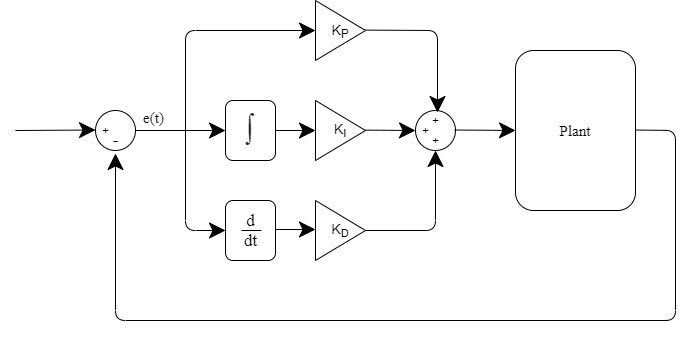
\includegraphics[width=\columnwidth]{PIDControl.png}%
	\caption{PID control block diagram.}%
	\label{fig:PIDControl}%
\end{figure}

PID control is comparatively simple compared to other techniques, but several studies suggest that it is generally effective for stabilising a UAV around a hovering setpoint, in the absence of large disturbances\cite{Bouabdallah2006}\cite{Pounds2010}\cite{Moussid2015}. \\

\subsection{Backstepping Control}\label{section:BacksteppingBackground}
The plant dynamics of a multi-rotor vehicle are inherently nonlinear, therefore nonlinear control techniques may be necessary to stabilise the vehicle. Backstepping control is a nonlinear recursive technique which is based upon Lyapunov stability. The mathematical background on the backstepping method in this section is largely based upon the work by Krsti\'c et al.\cite{Krstic1995}.

\subsubsection{Lyapunov Stability}
Direct Lyapunov theorem, as stated in Appendix B of \cite{Isidori1995}, considers a time invariant system of the form:
\[\dot{x}=f(x)\]
with $x\in\mathbb{R}^{n}$ and $f(x)$ smooth, with $f(0)=0$. If there exists a positive definite, proper and smooth function $V(x)$ which satisifies:
\[\frac{\partial V}{\partial x}f(x)<0\]
for all $x\neq0$, then the equilibrium of the system is globally asymptotically stable. This means that given any initial conditions, over time ($t\rightarrow\infty$) the system will approach its equilibrium point \cite{Chen1999}. 

Now, consider a time invariant nonlinear system with states $x$ and inputs $u$:
\begin{equation}\label{eqn:TISystem}
\dot{x}=f(x,u)
\end{equation}
with equilibrium at $x=0$. Following from Direct Lyapunov theorem, to stabilise such a system, a control law $u=\alpha(x)$ must be designed such that the equilibrium point of Equation \ref{eqn:TISystem} is globally asymptotically stable. To do this, a function $V(x)$ may be chosen as a candidate Lyapunov function. The control input, $\alpha(\textbf{\textit{x}})$, must then be chosen such that $\dot{V}(x)=\frac{\partial V}{\partial x}f(x,\alpha(x))$ is negative definite for all x. 

In order to apply this method to the tracking problem, the states of the system may be redefined as $z=x_{d}-x$, where $x_{d}$ represents the desired value of the $x$ states.









\section{State Estimation}

%Address the different techniques and evaluate their use in previous studies
%Kalman Filter...
%Extended Kalman Filter...
%EKF is similar to KF, but linearises a nonlinear system about the current estimated trajectory.

%UKF...


%Sensor Fusion/Multi-rate/Redundancy/fault detection

\subsection{Extended Kalman Filter}\label{section:EKFBackground}
There are two main steps to the EKF algorithm: predict and update.
The "predict" step first uses the state transition functions ($\textbf{\textit{f}}(x,u)$) with the previous state estimate ($\hat{\textbf{\textit{x}}}_{k-1}$) and the current input (\textbf{\textit{u}}) values. Then the covariance matrix (\textbf{\textit{P}}) is predicted using the Jacobian of the state transition function ($F$).

\begin{equation}
\begin{split}
\hat{x}_{k}^{-}&=f(\hat{x}_{k-1}, u_{k})\\
P_{k}^{-}&=F_{k}P_{k-1}F_{k}^{T}+Q_{k}
\end{split}
\end{equation}
where $Q_{k}$ represents the process noise covariance matrix.$F_{k}$ represents the Jacobian of the state transition function evaluated at ($\hat{x}_{k}^{-}$, $u_{k}$).  The "-" superscript denotes the initial estimate from the predict step.


The "update" step uses these predictions and compares them with the sensor measurements to achieve more accurate estimates.

\begin{equation}
\begin{split}
K_{k}&=P_{k}^{-}H_{k}^{T}(H_{k}P_{k}^{-}H_{k}^{T}+R_{k})^{-1}\\
\hat{x}_{k}&=\hat{x}_{k}^{-}+K_{k}\left[z_{k}-h(\hat{x}_{k}^{-})\right]\\
P_{k}&=(I-K_{k}H_{k})P_{k}^{-}
\end{split}
\end{equation}
where $z_{k}$ represents the sensor measurements, $h(\cdot)$ represents the measurement functions and I represents an identity matrix. $H_{k}$ represents the Jacobian of the measurement function evaluated at $\hat{x}_{k}^{-}$.

\subsection{Magnetometer}
The Earth's magnetic field vector varies with latitude, longitude, altitude and time. In order to effectively utilise magnetometer data to determine true north it may be necessary to have knowledge of the magnetic field vector's expected value at a particular location. The International Geomagnetic Reference Field or World Magnetic Model

\subsection{Barometer}\label{section:barometerBackground}
Air pressure varies with altitude, which allows barometric pressure sensors to be used in the estimation of relative height. The U.S. National Aeronautics and Space Administration (NASA) have developed a standard atmospheric model \cite{Oceanic1976}. According to this model, pressure as a function of height above sea level can be found using \eqref{eqn:baroFormula}, when temperature lapse rate is zero. Temperature lapse rate describes the rate at which temperature changes with altitude. 

\begin{equation}\label{eqn:baroFormula}
P=P_{b}exp\left[\frac{-g M (H-H_{b})}{R T_{b}}\right]
\end{equation}
where $P_{b}$, $T_{b}$ and $H_{b}$ are the reference values of pressure, temperature and height respectively. The subscript b is representative of one of seven layers of the atmosphere. H is the height at which pressure is calculated, g is gravitational acceleration, M is the molar mass of air and R is the universal gas constant. 

Assuming the UAV operates at altitudes below 11 km above sea level, the subscript b is 0. Within this operating region the reference values are: $P_{0}=101 325$ Pascals, $T_{0}=288.15$ Kelvin and $H_{0}=0$ metres,
 

\section{Chapter Summary}
This chapter has provided the technical background necessary for the development in the following chapters. A comprehensive review of current literature has also been established in order to reveal the more effective methods and the gaps in current research.



\clearpage


